\documentclass[10pt,letterpaper]{article}
\usepackage[utf8]{inputenc}
\usepackage{amsmath}
\usepackage{amsfonts}
\usepackage{amssymb}
\usepackage{graphicx}
\usepackage{siunitx}
\DeclareSIUnit{\torr}{torr}
\sisetup{retain-unity-mantissa = false}
\usepackage{booktabs}

\author{W. Schreyer, S. Morawetz}
\title{Fall run 2018 -- analysis report}
\begin{document}

\maketitle

\tableofcontents

\section{Introduction}

This document describes several analyses of the data taken during the 2018 run of the UCN source at TRIUMF, covering measurements of
\begin{itemize}
\item transmission through guide components
\item storage lifetime in the source, and
\item storage lifetime in guide components.
\end{itemize}

All these experiments are performed in cycles. Each cycle contains several periods, typically starting with an irradiation period, during which the target is irradiated with protons and ultracold neutrons are produced. This can be followed by up to 9 more periods, like storage or detection periods. For each period, up to 8 UCN components like valves or spin flippers can be to set different states. The last (11th) period covers the time until the next irradiation and cycle starts.

Cycles with different period durations and valve settings can be grouped in supercycles, which can be repeated several times. Cycles of one experiment can be spread over several Midas runs.

Two UCN detectors were used throughout the run. A Li6 detector, detecting scintillation light of UCN captured in $^6$Li-enriched glass, and a He3 detector, detecting gas discharges due to UCN captured by $^3$He. Experiments can use either detector alone or both at the same time.


\section{Preparation of raw detector data}

The Li6 detector uses two values to determine if a detected event was actually caused by a UCN: ``PSD'' based on the pulse shape of the event and $Q_\mathrm{long}$, the charge collected during a \SI{200}{\nano\second} window after the event trigger. An event is considered a UCN if
\begin{equation}
\mathrm{PSD} > 0.3
\end{equation}
and
\begin{equation}
Q_\mathrm{long} > 2000.
\end{equation}

The He3 detector considers an event to be a UCN if the charge collected after the event trigger
\begin{equation}
Q_\mathrm{short} > 300.
\end{equation}

\section{Transmission measurements}

Transmission measurements are experiments with two periods per cycle. An irradiation period, where UCN are produced and a small percentage is detected in the He3 detector connected to a monitoring port, while a valve downstream of the He3 detector is closed. And a counting period, where the UCN valve is opened and UCN transmitted through components downstream of the valve are detected in the Li6 detector.

The number of UCN detected in the He3 ``monitor'' detector during irradiation is a direct measure of the number of UCN actually produced by the source. The ratio of the number of UCN detected in the Li6 detector during the detection period to the ``monitor counts'' therefore is directly proportional to how many of the produced UCN could be transmitted through the guide components downstream of the valve. To compare the transmission through guide components in two different setups, we can divide the ratios from each of those setups.

A constant background rate $b^\mathrm{Li6}$ (see section \ref{sec:background}) is subtracted from the number of UCN counted in the Li6 detector during counting $C^\mathrm{Li6}_\mathrm{counting}$:
\begin{equation}
N^\mathrm{Li6}_\mathrm{counting} = C^\mathrm{Li6}_\mathrm{counting} - b^\mathrm{Li6} \cdot t_\mathrm{counting},
\end{equation}
with an uncertainty
\begin{equation}
\Delta N^\mathrm{Li6}_\mathrm{counting} = \sqrt{ \sqrt{C^\mathrm{Li6}_\mathrm{counting}}^2 + \left( \Delta b^\mathrm{Li6} \cdot t_\mathrm{counting} \right)^2}.
\end{equation}
Then the background-corrected count $N^\mathrm{Li6}_\mathrm{counting}$ is divided by the number of UCN detected in the He3 detector during the irradiation period $N^\mathrm{He3}_\mathrm{irradiation}$
\begin{equation}
R = \frac{N^\mathrm{Li6}_\mathrm{counting}}{N^\mathrm{He3}_\mathrm{irradiation}},
\end{equation}
with an uncertainty
\begin{equation}
\Delta R = \sqrt{ \left( \frac{\Delta N^\mathrm{Li6}_\mathrm{counting}}{N^\mathrm{He3}_\mathrm{irradiation}} \right)^2 + \left( \sqrt{N^\mathrm{He3}_\mathrm{irradiation}} \frac{N^\mathrm{Li6}_\mathrm{counting}}{{N^\mathrm{He3}_\mathrm{irradiation}}^2} \right)^2  },
\end{equation}
The He3 detector is assumed to be background-free\footnote{The expected number of background counts is about 6, while the total count during irradiation varies between 2000 and 4000}.

\begin{figure}
\centering
\includegraphics[width=\textwidth,page=1]{{"../transmission/TCN18-045 (IV2+UGD22+IV3, O-rings in)"}.pdf}
\caption{Ratio of Li6 counts to He3 counts for all cycles of transmission experiment TCN18-045, fitted with a constant function. The legend shows the $\chi^2/\nu$ of the fit, the average ratio $\bar{R}$, and its uncertainty.}
\label{fig:transmission}
\end{figure}

The ratios for all cycles are plotted using ROOT. A $\chi^2$ fit of a constant function over all cycles is used to determine the average $\bar{R}$ and its uncertainty $\Delta \bar{R}$, see figure \ref{fig:transmission}.

The relative transmission $T$ of one experiment compared to another is
\begin{equation}
T = \frac{\bar{R}_1}{\bar{R}_2}
\end{equation}
with the uncertainties for each $\bar{R}$ scaled by the $\chi^2$ per degrees of freedom $\nu$ from the fit:
\begin{equation}
\Delta T = T \sqrt{ \left( \frac{\Delta \bar{R}_1 \chi_1^2}{\bar{R}_1 \nu_1} \right)^2 + \left( \frac{\Delta \bar{R}_2 \chi_2^2}{\bar{R}_2 \nu_2} \right)^2 }.
\end{equation}

\subsection{Time of flight}

The transmission experiments also allow us to study how transmission changes over time. Following the same scheme shown above, we look at the background-corrected number of counts detected in the Li6 detector in narrow time bins $\Delta t = t_{i + 1} - t_i$ after the valve opened
\begin{equation}
N^\mathrm{Li6}_{t_i} = C^\mathrm{Li6}_{t_i} - b^\mathrm{Li6} \cdot \Delta t,
\end{equation}
and normalize them to the number of UCN detected in the He3 detector during irradiation
\begin{equation}
R_{t_i} = \frac{N^\mathrm{Li6}_{t_i}}{N^\mathrm{He3}_\mathrm{irradiation}}.
\end{equation}

\begin{figure}
\centering
\includegraphics[width=\textwidth,page=2]{{"../transmission/TCN18-045 (IV2+UGD22+IV3, O-rings in)"}.pdf}
\caption{Rate in the Li6 detector after opening the valve during transmission experiment TCN18-045, normalized to the He3 detector and averaged over all cycles.}
\label{fig:time_of_flight}
\end{figure}

The resulting time-binned histogram is averaged over all cycles using ROOT, see figure \ref{fig:time_of_flight}.

\begin{figure}
\centering
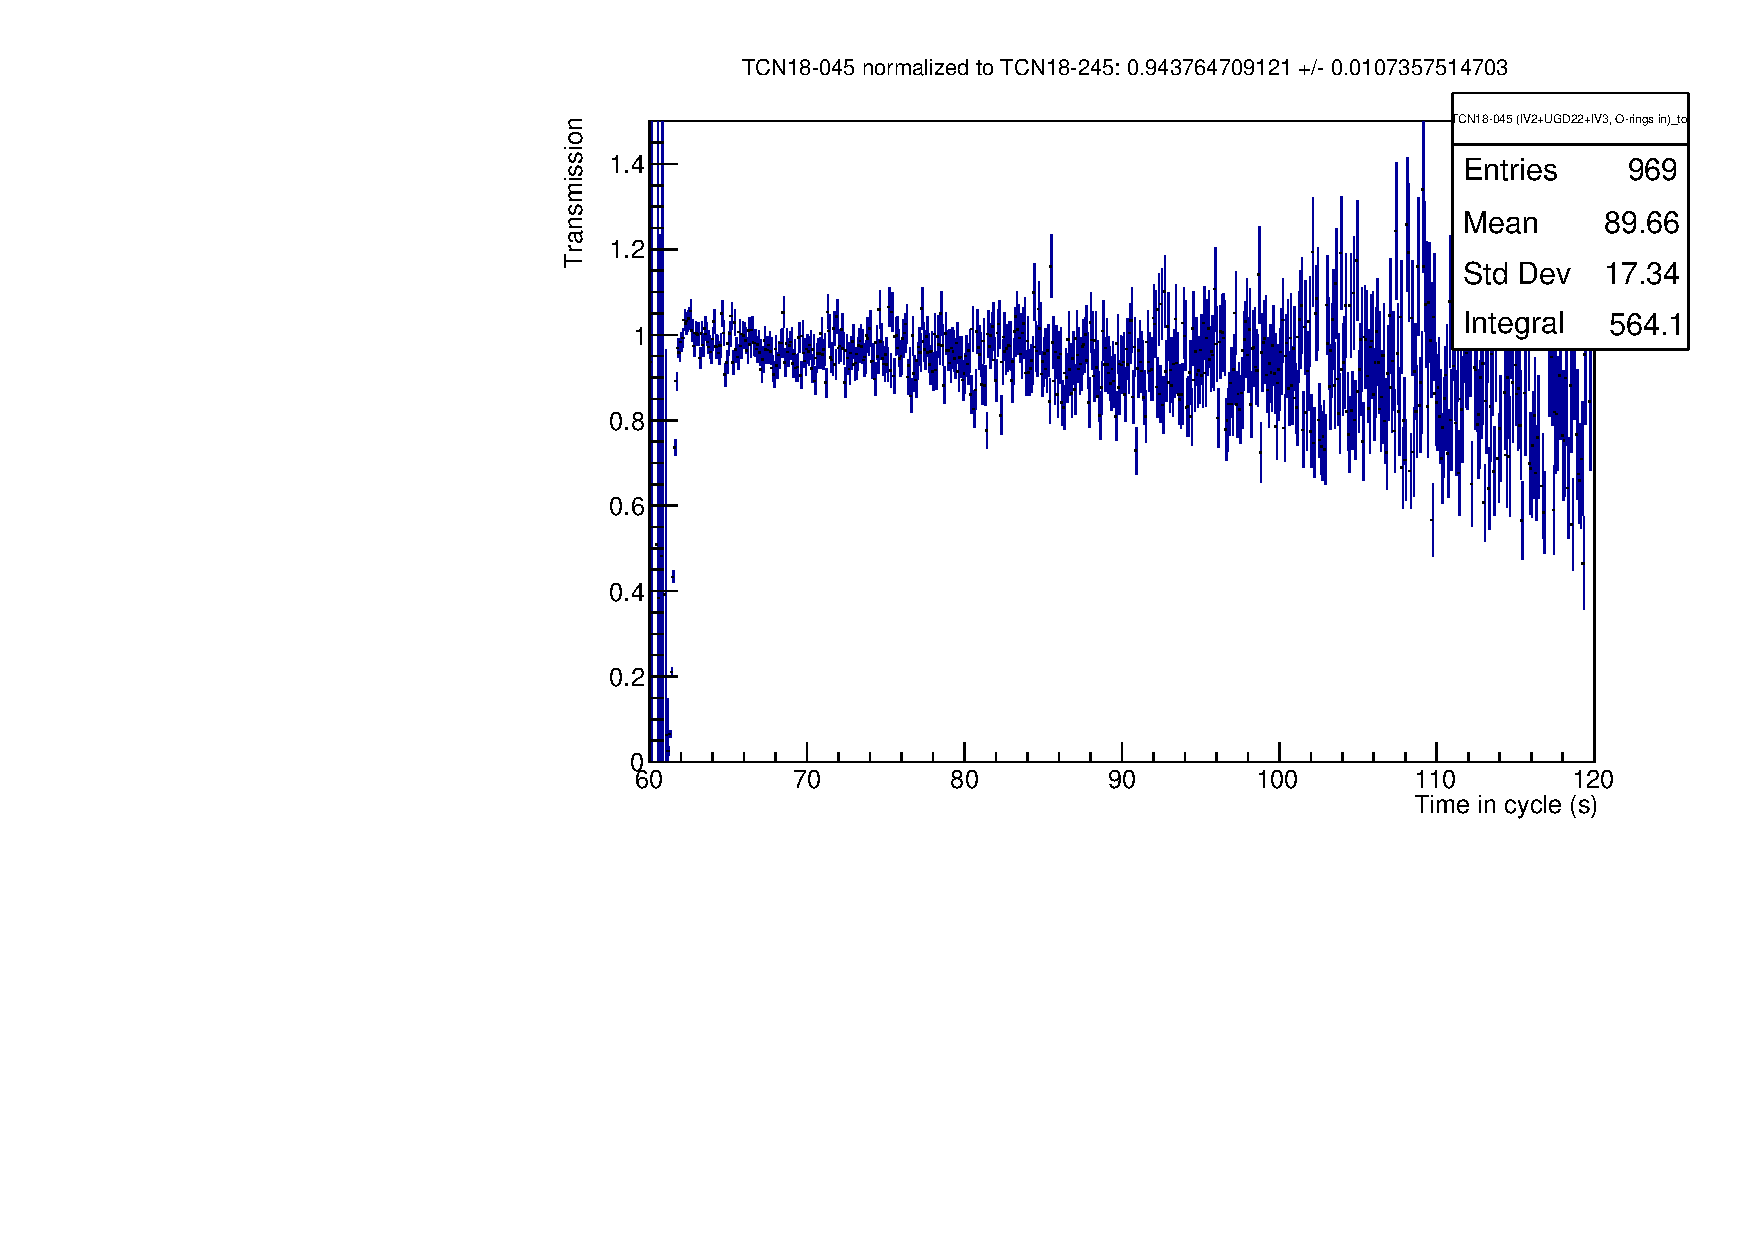
\includegraphics[width=\textwidth,page=1]{../transmission/TCN18-045_TCN18-245.pdf}
\caption{Ratio of normalized rates in experiment TCN18-045 and TCN18-245. The title contains the total relative transmission $T$.}
\label{fig:time_of_flight_normalized}
\end{figure}

Dividing the histograms from two different transmission experiments shows how the relative transmission changes over time, see figure \ref{fig:time_of_flight_normalized}.

\subsection{Excluded cycles}

Individual cycles can be excluded from the analyzed transmission data if
\begin{itemize}
\item the beam current dropped below \SI{0.1}{\micro\ampere} (10 cycles);
\item the beam current fluctuated by more than \SI{0.02}{\micro\ampere} (10 cycles);
\item the last period does not contain any Li6 events, i.e. the run was aborted at some point during this cycle (34 cycles);
\item the He3 detector detected less than 1000 UCN during irradiation (6 cycles);
\item the ion gauge IG6 read a pressure between \SIlist{1e-7;1e-2}{\torr}, indicating that it was on, causing additional background in the Li6 detector (62 cycles);
\item the Li6 detector detected an average rate below \SI{10}{\hertz} during the counting period (0 cycles); or
\item the Li6 detector detected a large background rate above \SI{10}{\hertz} during the irradiation period (4 cycles).
\end{itemize}

In total, 126 out of 541 cycles were excluded. All cycles of experiments TCN18-029 (run 934) and TCN18-080 (run 973) had to be discarded, due to IG6 being on.

\subsection{Results}

\begin{table}
\centering
\caption{Results of transmission experiments. If not otherwise noted, all transmission measurements were performed with the listed guides between IV2 and IV3, the IVs' O-rings pointing towards each other, and a 90$^\circ$ elbow downstream of IV3. The $\chi^2$ gives an indication of how well the data fits the assumption that the ratio $R$ stays constant over all cycles in each experiment.}
\begin{tabular}{l r r r p{0.4\textwidth}}
\toprule
Experiment & Run & $\bar{R}$ & $\chi^2/\nu$ & Description \\
\midrule
TCN18-031 & 938 & $12.92 \pm 0.06$ & 1.90 & IV2 + UGD17 + elbow \\
TCN18-035 & 944 & $11.81 \pm 0.06$ & 1.23 & UGD22, O-rings of IVs pointing away from each other \\
TCN18-045 & 954 & $11.75 \pm 0.06$ & 2.04 & UGD22 \\
TCN18-053 & 985 & $11.27 \pm 0.06$ & 1.64 & burst disk + UGD2 \\
TCN18-085 & 973 & $11.29 \pm 0.06$ & 1.66 & UGD22 + 19 (NiP) \\
TCN18-090 & 1000 & $10.96 \pm 0.06$ & 1.48 & UGD22 + UGA11 + UGG3 + UGA5 \\
TCN18-290 & 1009 & $11.08 \pm 0.07$ & 1.56 & UGD22 + UGA5 + UGG3 + UGA6 \\
TCN18-060 & 1013 & $11.38 \pm 0.06$ & 1.19 & UGD10 + 17 + 11 \\
TCN18-065 & 1054 & $11.20 \pm 0.06$ & 1.19 & SCM warm bore \\
TCN18-265 & 1081 & $6.51 \pm 0.04$ & 0.62 & SCM warm bore with foil \\
TCN18-115 & 1125 & $6.95 \pm 0.04$ & 2.57 & UGD22 + 2 + Ti foil \\
TCN18-245 & 1129 & $12.45 \pm 0.07$ & 0.65 & UGD22 (repeat) \\
TCN18-480 & 1131 & $12.12 \pm 0.07$ & 0.80 & UGD22 + 2 \\
TCN18-057 & 1141 & $11.73 \pm 0.06$ & 1.42 & vent spider + UGD2 \\
\midrule
\multicolumn{5}{l}{Experiments at high position:} \\
TCN18-302 & 1165 & $16.07 \pm 0.07$ & 1.89 & IV2 + elbow + UGD10 + 18 \\
TCN18-240 & 1176 & $9.95 \pm 0.05$ & 1.79 & IV2 + elbow + UGD10 + Al foil + UGD18 \\
TCN18-215 & 1181 & $7.14 \pm 0.04$ & 1.57 & UGD22 + 20 + Ti foil \\
TCN18-380 & 1188 & $15.8 \pm 0.08$ & 3.07 & UGD22 + 20 \\
TCN18-310 & 1192 & $17.12 \pm 0.07$ & 1.56 & UGD22 + 20, smooth elbow \\
\bottomrule
\end{tabular}
\label{tab:transmission}
\end{table}

\begin{table}
\centering
\caption{Comparison of transmission experiments.}
\begin{tabular}{l r r p{0.4\textwidth}}
\toprule
Experiment & Reference & $T$ & Description \\
\midrule
TCN18-045 & TCN18-245 & $0.944 \pm 0.010$ & Comparison of reference measurements \\
TCN18-035 & TCN18-031 & $0.912 \pm 0.010$ & UGD22+IV3 compared to UGD17\\
TCN18-045 & TCN18-035 & $0.994 \pm 0.013$ & Flipping IV2 and IV3\\
TCN18-053 & TCN18-045 & $0.959 \pm 0.013$ & Replacing UGD22 with burst disk and UGD2 \\
TCN18-085 & TCN18-045 & $0.960 \pm 0.014$ & Adding UGD19 (NiP) \\
TCN18-090 & TCN18-045 & $0.932 \pm 0.013$ & Adding UGG3 with UGA11+3 \\
TCN18-290 & TCN18-045 & $0.943 \pm 0.013$ & Adding UGG3 with UGA5+6\\
TCN18-060 & TCN18-045 & $0.969 \pm 0.012$ & Replacing UGD22 with UGD10 + 17 + 11 \\
TCN18-065 & TCN18-045 & $0.953 \pm 0.012$ & Replacing UGD22 with SCM warm bore \\
TCN18-265 & TCN18-065 & $0.581 \pm 0.004$ & Adding foil to SCM warm bore \\
TCN18-115 & TCN18-480 & $0.573 \pm 0.009$ & Adding Ti foil \\
TCN18-480 & TCN18-245 & $0.974 \pm 0.006$ & Adding UGD2 \\
TCN18-057 & TCN18-245 & $0.942 \pm 0.008$ & Replacing UGD22 with vent spider and UGD2 \\
\midrule
\multicolumn{4}{l}{Experiments at high position:} \\
TCN18-240 & TCN18-302 & $0.619 \pm 0.007$ & Adding Al foil \\
TCN18-215 & TCN18-380 & $0.451 \pm 0.008$ & Adding Ti foil \\
TCN18-310 & TCN18-380 & $1.082 \pm 0.019$ & Replacing kinked with smooth elbow\\
\bottomrule
\end{tabular}
\label{tab:transmission_comparison}
\end{table}

Table \ref{tab:transmission} lists the results of the individual transmission experiments and table \ref{tab:transmission_comparison} compares several.

The most striking result is that the identical reference experiments TCN18-045 and TCN18-245 performed at different times do not agree. This suggests that some time between runs 954 and 1129 either the transmission, the detector efficiencies, the geometry upstream of IV2, or the UCN spectrum changed. Unfortunately another test of repeatability, TCN18-080, which was set up identically to TCN18-480, had to be discarded.

For now, the earlier transmission experiments up to run 1081 are compared to TCN18-045 and the later ones from run 1131 are compared to TCN18-245.

The ratio of time-of-flight histograms (Fig. \ref{fig:time_of_flight_normalized}) shows that transmission in the first few seconds of TCN18-045 is lower than in TCN18-245, suggesting that there also is some timing discrepancy.

\subsection{SCM transmission}

We equipped the superconducting polarizer magnet (SCM) with a ``warm'' bore with an inner diameter of \SI{85}{\milli\meter} and an \SI{0.1}{\milli\meter} thick AlMg3 foil in the center. Due to the tight fit of the guide through the cold superconducting magnet coil the foil could only be clamped between two narrow surfaces and was stripped out when we accidentally produced a pressure difference across the foil while pumping the guide. Hence, we did the first transmission measurements without a foil. We were able to insert a new foil soldered onto a thin stainless-steel ring later on and performed the same measurements with the foil inserted.

As seen in table~\ref{tab:transmission_comparison}, adding the warm bore without the foil reduced transmission to the Li6 detector by \SI{5}{\percent}, and only by \SI{2}{\percent} compared to stainless-steel guides with the same total length (TCN18-060), despite the gaps in the Wilson-style flanges holding the bore.

\begin{figure}
\centering
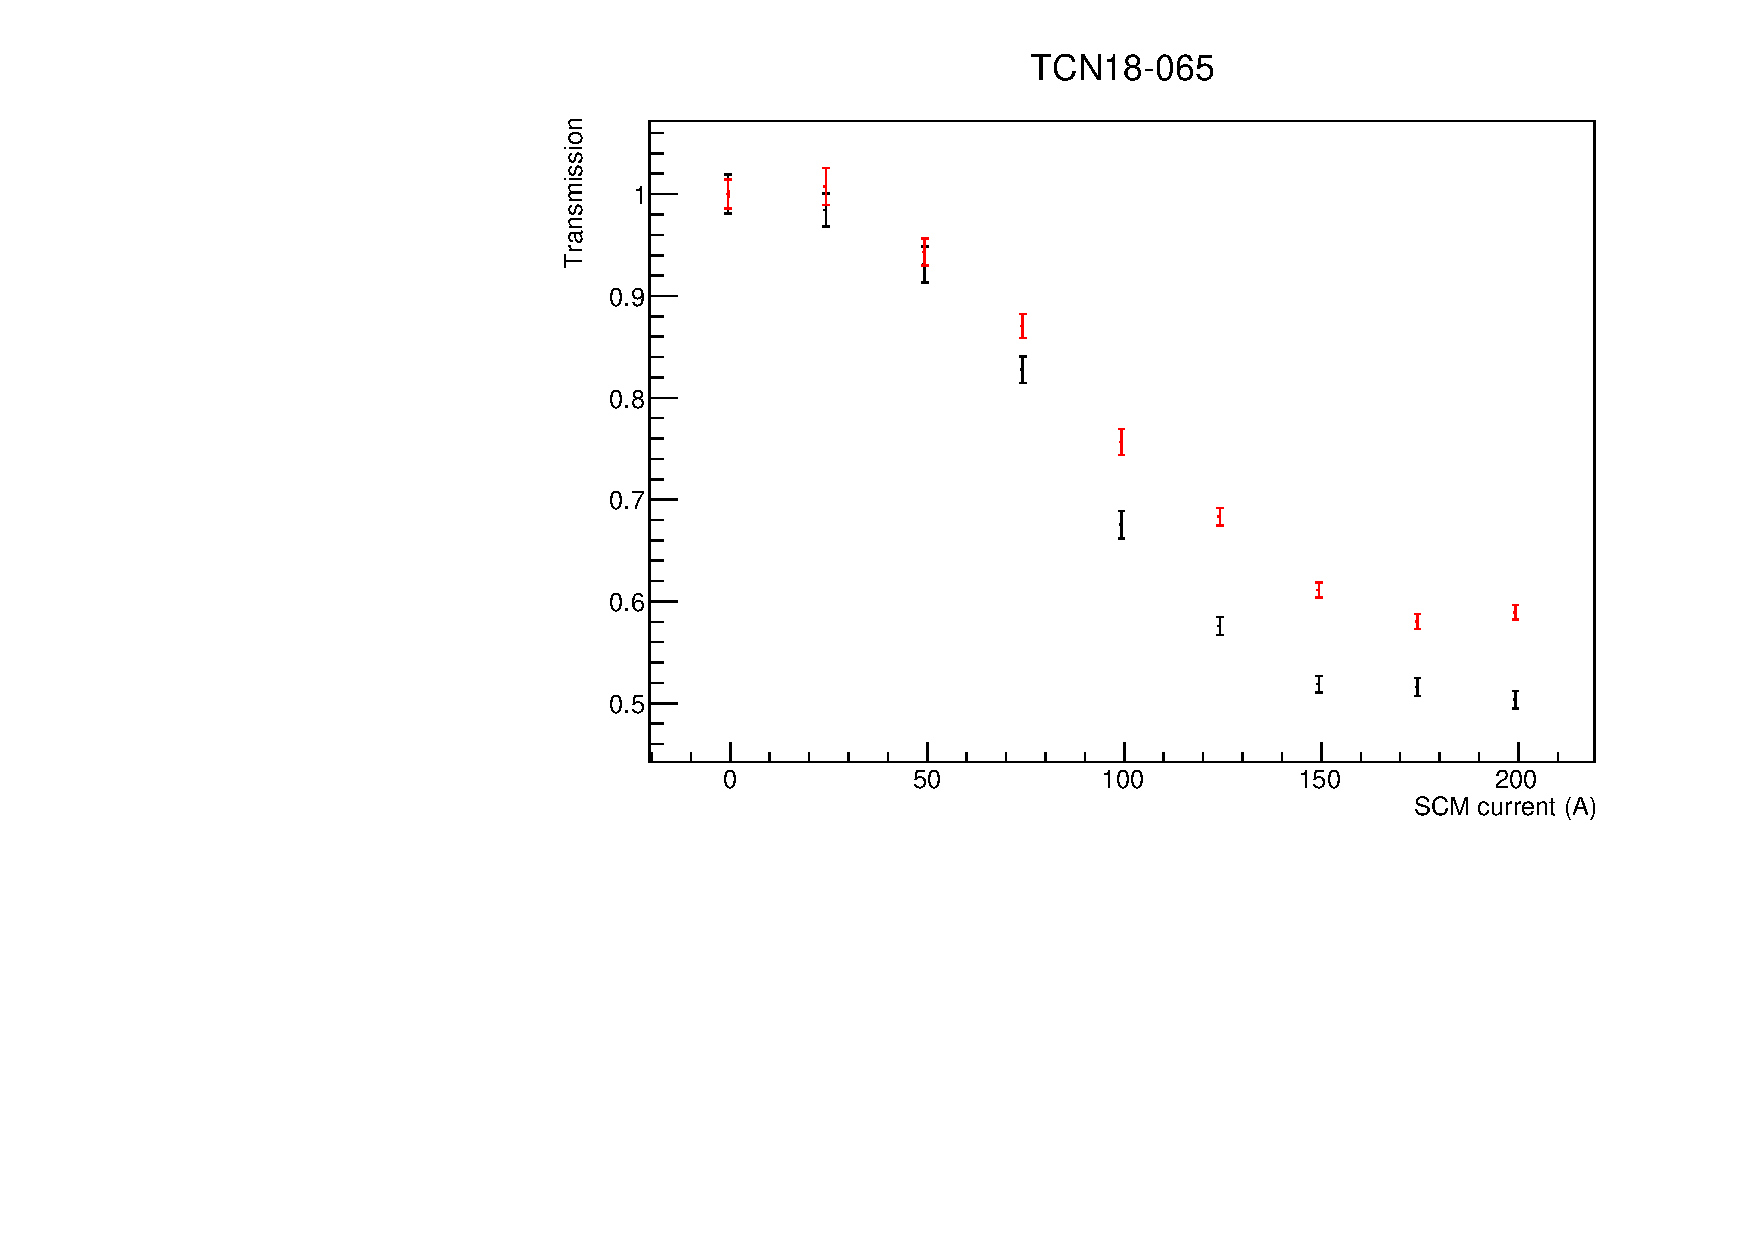
\includegraphics[width=\textwidth,page=1]{../transmission/TCN18-065.pdf}
\caption{Transmission $T$ through the warm bore while the SCM is powered with different currents, compared to transmission while unpowered.}
\label{fig:SCMtransmission_nofoil}
\end{figure}

When the current in the SCM magnet is increased the magnetic field $B$ acts as a potential wall or trough with $V = \pm \SI{60.3}{\nano\electronvolt\per\tesla} \cdot B$, depending on the UCN's spin polarization. UCNs with the wrong polarization (low-field seekers) cannot penetrate the potential if their energy is too low, so at higher currents a larger part of their spectrum is not transmitted and the total transmission drops.

At the maximum current of \SI{200}{\ampere} the central field was measured as \SI{3.79}{\tesla}, sufficient to polarize UCNs with energies up to \SI{229}{\nano\electronvolt}. Due to the geometry of the source and UCN guides, we expect an energy range for UCNs roughly between \SIlist{90;180}{\nano\electronvolt}. This is confirmed by the transmission curve (Fig. \ref{fig:SCMtransmission_nofoil}) starting to drop at about \SI{50}{\ampere}, corresponding to $V = \SI{70}{\nano\electronvolt}$ and leveling out at \SI{150}{\ampere}, corresponding to $V = \SI{170}{\nano\electronvolt}$. However, it does not drop to a transmission of \SI{50}{\percent}, as we would expect if all low-field seekers are stopped by the magnetic field.

\begin{figure}
\centering
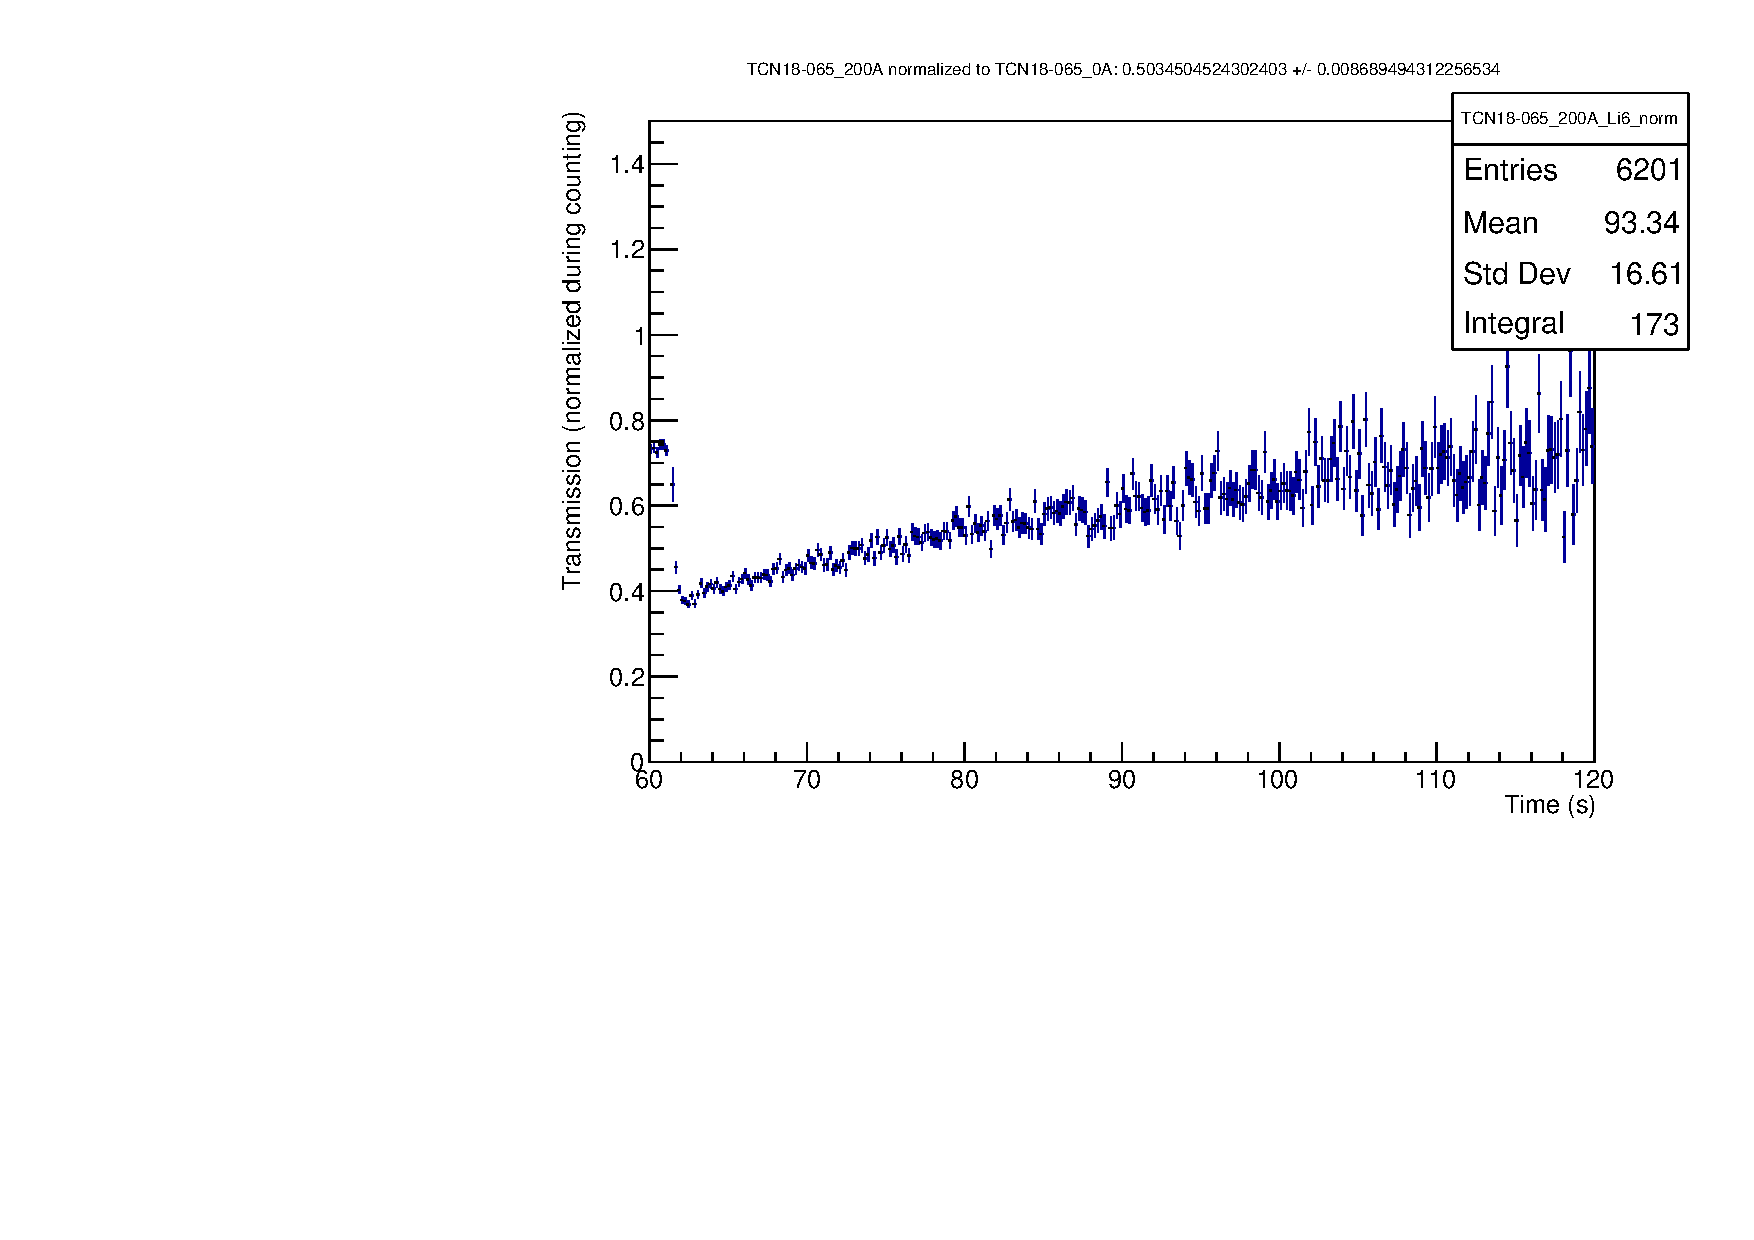
\includegraphics[width=\textwidth,page=1]{../transmission/TCN18-065_200A_TCN18-065_0A.pdf}
\caption{Normalized rate in the Li6 detector with the SCM at full current divided by the rate with no current.}
\label{fig:SCMtof_nofoil}
\end{figure}

When comparing the UCN rates over time (Fig. \ref{fig:SCMtof_nofoil}), we see that the initial transmission at full current indeed drops to \SI{50}{\percent} of the transmission at no current, and then slowly increases. This suggests that the low-field seekers trapped upstream of the SCM slowly depolarize and leak through the SCM.

\begin{figure}
\centering
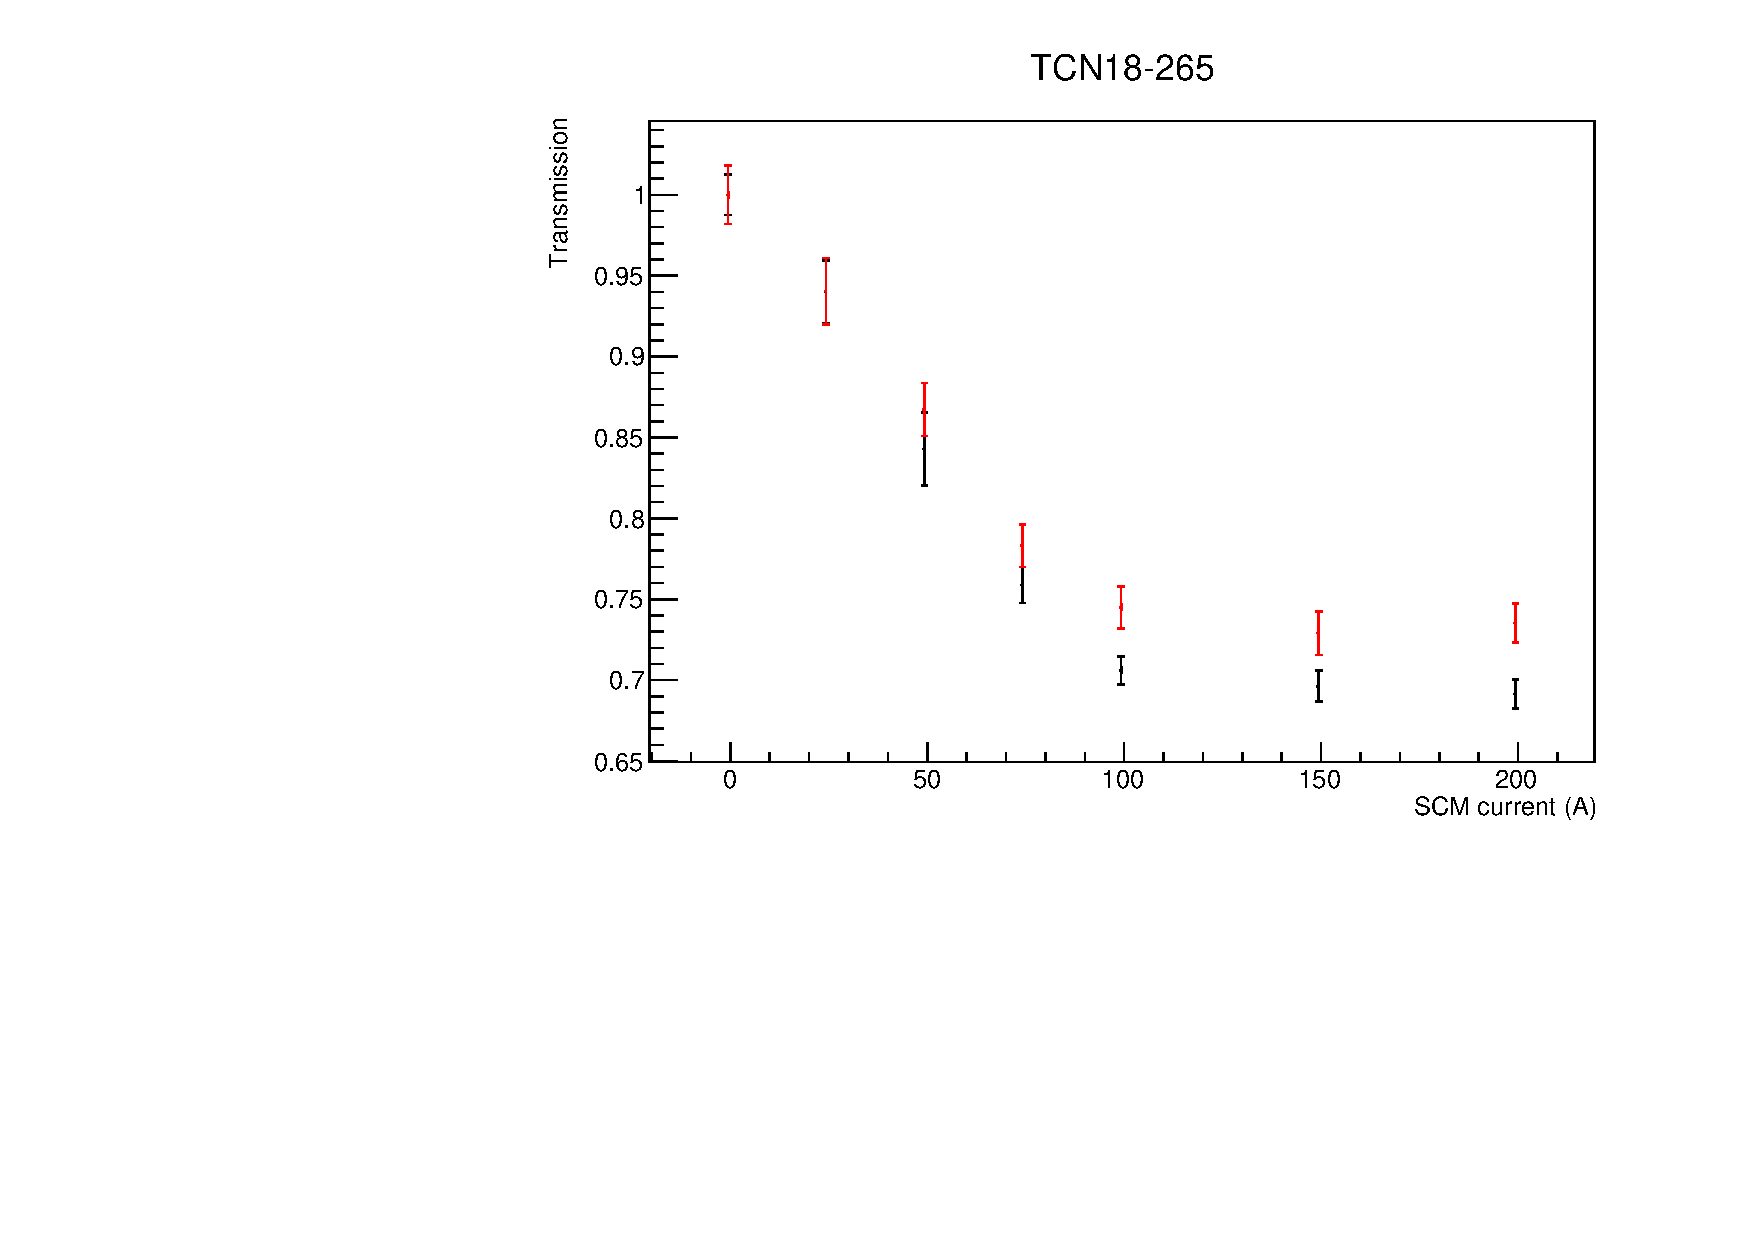
\includegraphics[width=\textwidth,page=1]{../transmission/TCN18-265.pdf}
\caption{Transmission $T$ through the warm bore with foil while the SCM is powered with different currents, compared to transmission while unpowered.}
\label{fig:SCMtransmission_foil}
\end{figure}

When we inserted the foil, the transmission through the SCM with no current dropped by \SI{42}{\percent} (Table \ref{tab:transmission_comparison}). This drop is slightly higher than what we measured when adding the foil in experiment TCN18-240, most likely due to the stainless-steel ring and solder.

\begin{figure}
\centering
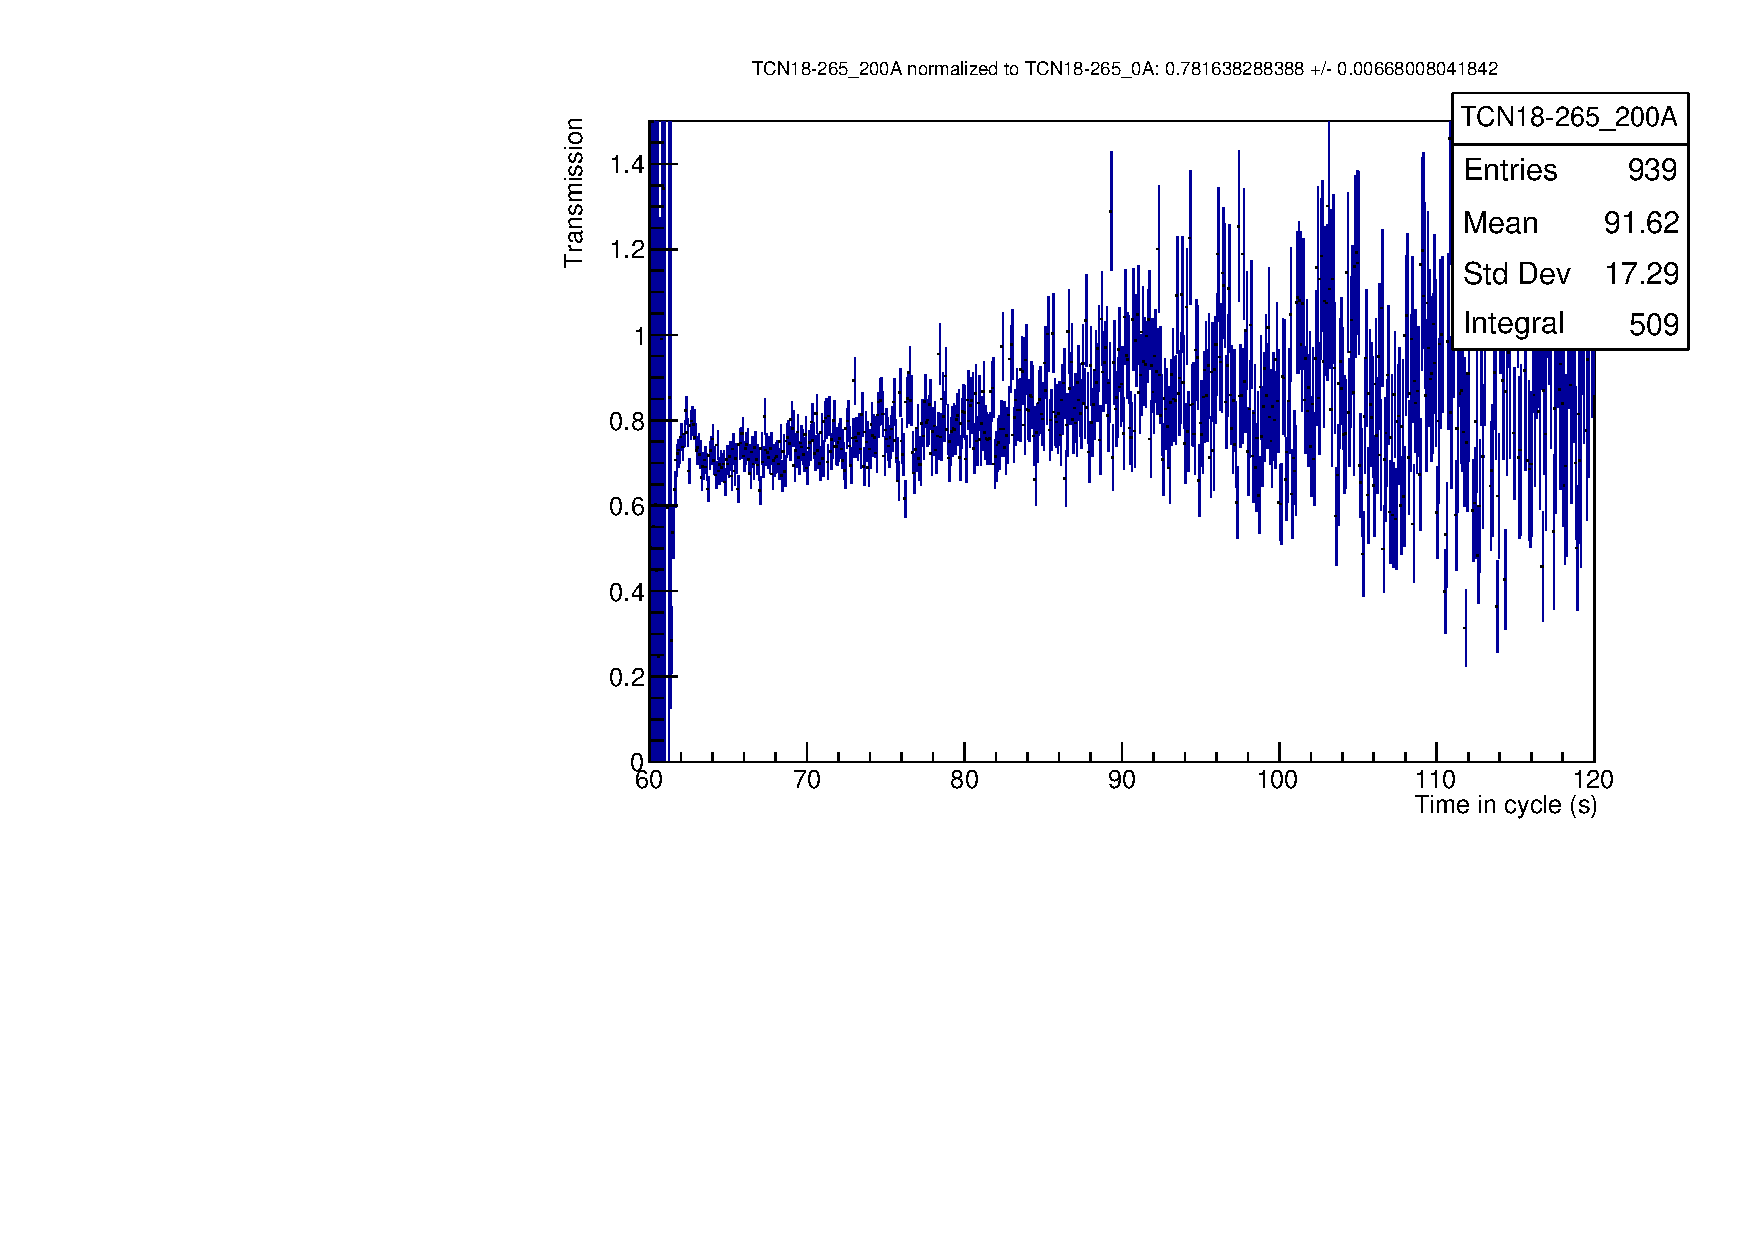
\includegraphics[width=\textwidth,page=1]{../transmission/TCN18-265_200A_TCN18-265_0A.pdf}
\caption{Normalized rate in the Li6 detector with the SCM at full current divided by the rate with no current, with the foil inserted.}
\label{fig:SCMtof_foil}
\end{figure}

With the foil, the transmission curve starts to drop and level out at lower currents, since the aluminium foil adds its Fermi potential of \SI{54}{\nano\electronvolt} to the potential barrier. It also levels off at a higher relative transmission of \SI{78}{\percent} and the initial time-resolved transmission at full current is much higher at \SI{70}{\percent} (Fig. \ref{fig:SCMtof_foil}), since the magnetic field accelerates the high-field seekers and reduces their absorption in the foil, counteracting the loss of low-field seekers.

These effects have to be confirmed in simulation.




\section{Thermal neutron detector}

The output on this device is time-averaged(?), and therefore it will take some time before the reading is accurate. Therefore, some ``buffer'' time is requied until the reading stabilizes. Although it will sometimes stabilize more quickly, this buffer time is set at \SI{30}{\second}. If a cycle is completed before this time is reached (i.e. the beam on duration is less than \SI{30}{\second}), then that cycle is discarded. All of the LND readings between this buffer time and the moment the beam goes off are averaged, and that plateau is reported as the LND reading. If the cycle ends before the beam goes off, but after \SI{30}{\second}, then all times beyond \SI{30}{\second} are averaged to get the LND reading. An example of the LND reading over time is shown in Fig \ref{fig:LNDplateau}.

\begin{figure}
\centering
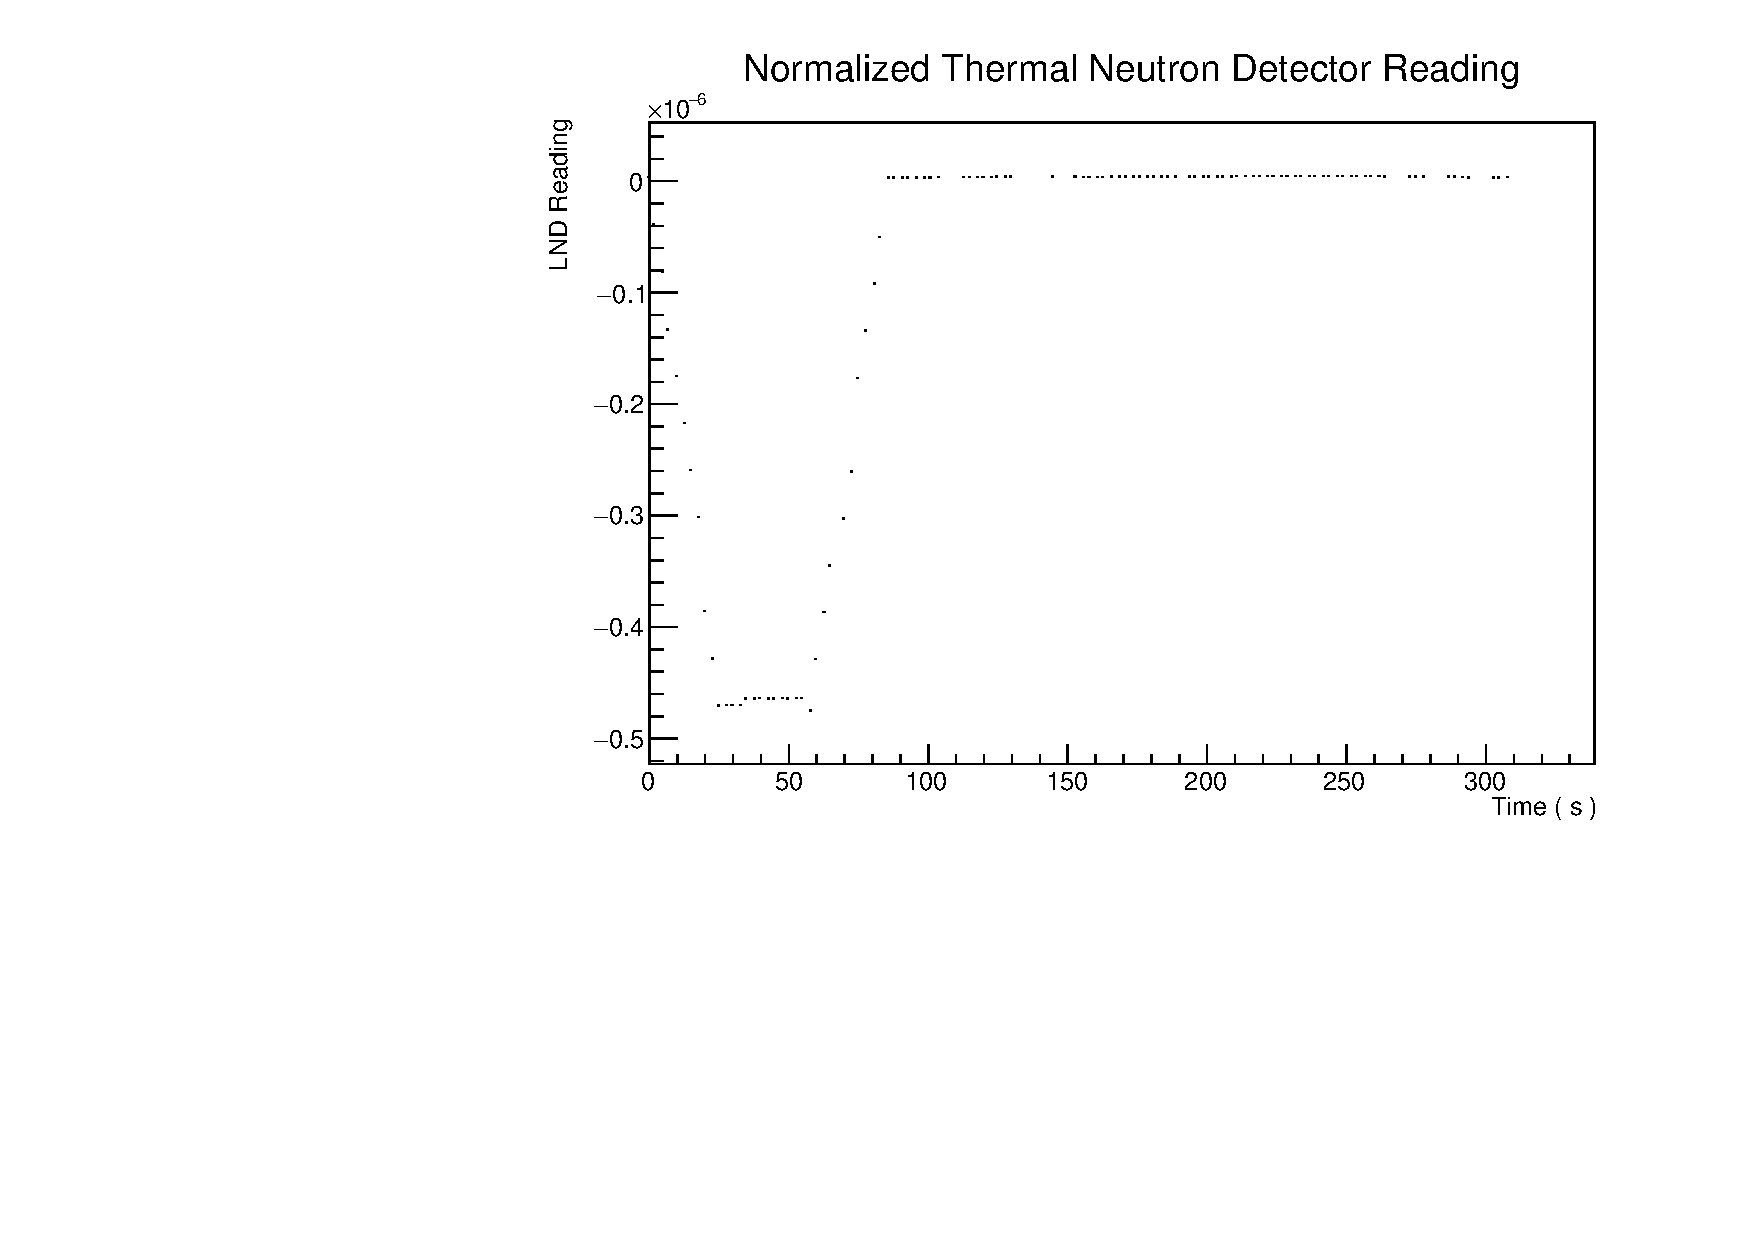
\includegraphics[width=\textwidth,page=1]{../thermal_neutron_detector/lndReadingVsTimeTCN18-042.pdf}
\caption{Thermal neutron detector device reading. Notice the current rising prior to reading a plateau, stabilizing, and then dropping off}
\label{fig:LNDplateau}
\end{figure}

Not every cycle has reliable data, however. Cycles in which the LND reading drops below \SI{0.1}{\micro\ampere}, or those where the beam fluctuates with a standard deviation of more than \SI{0.02}{\micro\ampere} are discarded. There is also a period from November 16 to November 26 during which the average LND reading jumps up by \approx\SI{0.3}{\micro\ampere}. The cause of this change is uncertain, but it is highly likely that this was due to an issue with the DAQ hardware, and therefore not due to some sudden physical change. Finally, there are some cycles in which the device was disabled, which are also discarded. The remaining, valid cycles are binned in and plotted in Fig \ref{fig:LNDhist}, with a Gaussian fit.

\begin{figure}
\centering
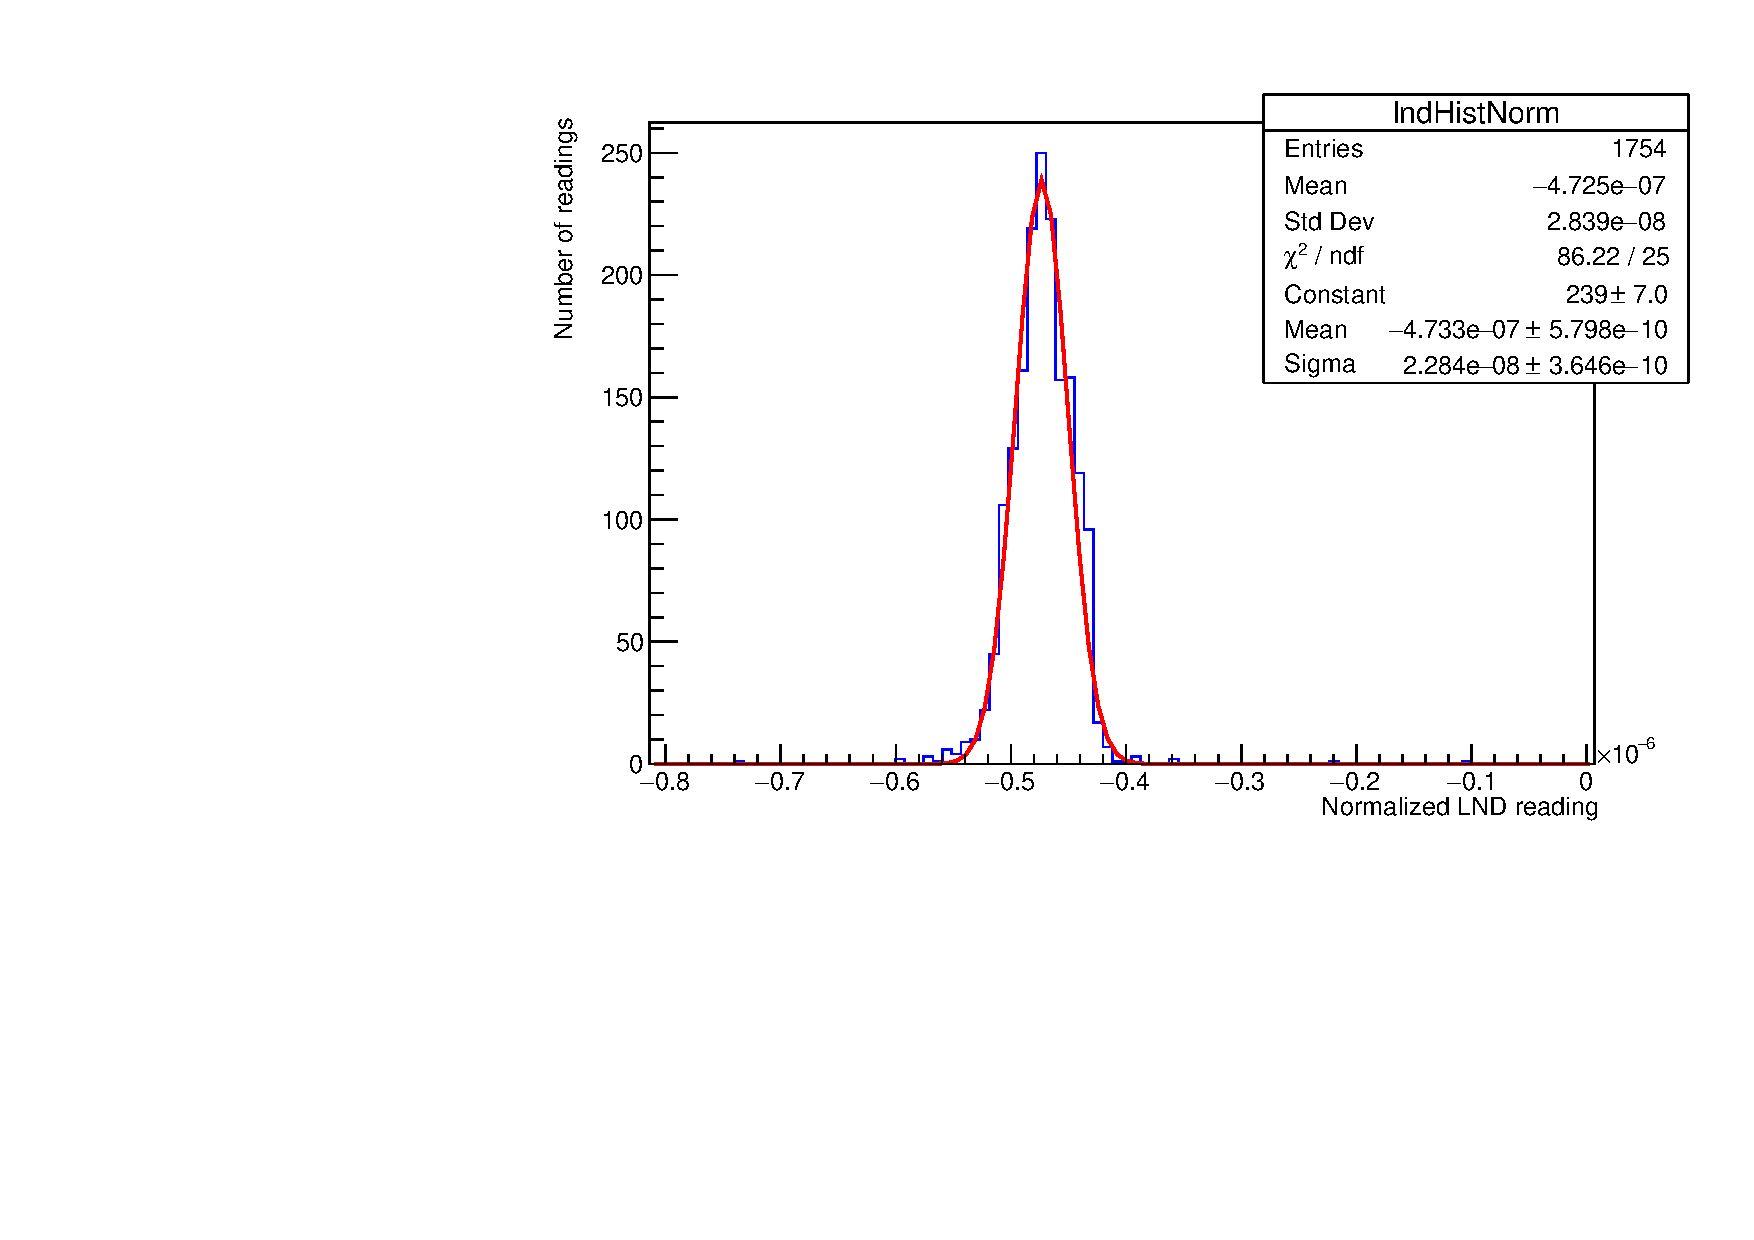
\includegraphics[width=\textwidth,page=1]{../thermal_neutron_detector/lndHist.pdf}
\caption{LND reading histogram with Gaussian fit}
\label{fig:LNDhist}
\end{figure}



\section{Steady state count rate}

In two different cycles, the VAT valve is opened and UCN are continually produced. In one cycle, the source is cooled down during this time, and in the other it is warmed up. The goal of this study is to analyze how the temperature affects the count rates of UCN in the Li-6 and He-3 detectors, and to determine which of the possible temperature measurement devices (TS11, TS12, TS14, TS16 or PG9) gives the most accurate temperature measurement. In the case of PG9, the pressure measurement is converted into a temperature with a temperature-vapour pressure correlation.

To ensure that the data is reliable, several cuts are made. Firstly, every during every period from when the beam current drops below \SI{0.9}{\micro\ampere}, until \SI{60}{\second} after it returns above \SI{0.9}{\micro\ampere}, the data is discarded. Additionally, at any instant in which the VAT valve IV1 is closed, the data is discarded. There are two devices, PG9L and PG9H, which read the vapour pressure. PG9L is a more accurate reading below \SI{2}{\milli\torr}, whereas PG9H is more accurate above \SI{2}{\milli\torr}. Therefore, the reading from PG9L is used when it reads below that threshold, and PG9H is used otherwise. Finally, the experimentally determined background for the Li-6 detector is subtracted, and the count rates are normalized to beam current.

Two separate plots of count rate vs temperature are made, for warming up, Fig \ref{fig:steadyWarm}, and cooling down, Fig \ref{fig:steadyCool}. The count rate is plotted as a function of temperature as measured by each of the different devices. It would appear as though PG9 produces the most accurate measurement.

\begin{figure}
\centering
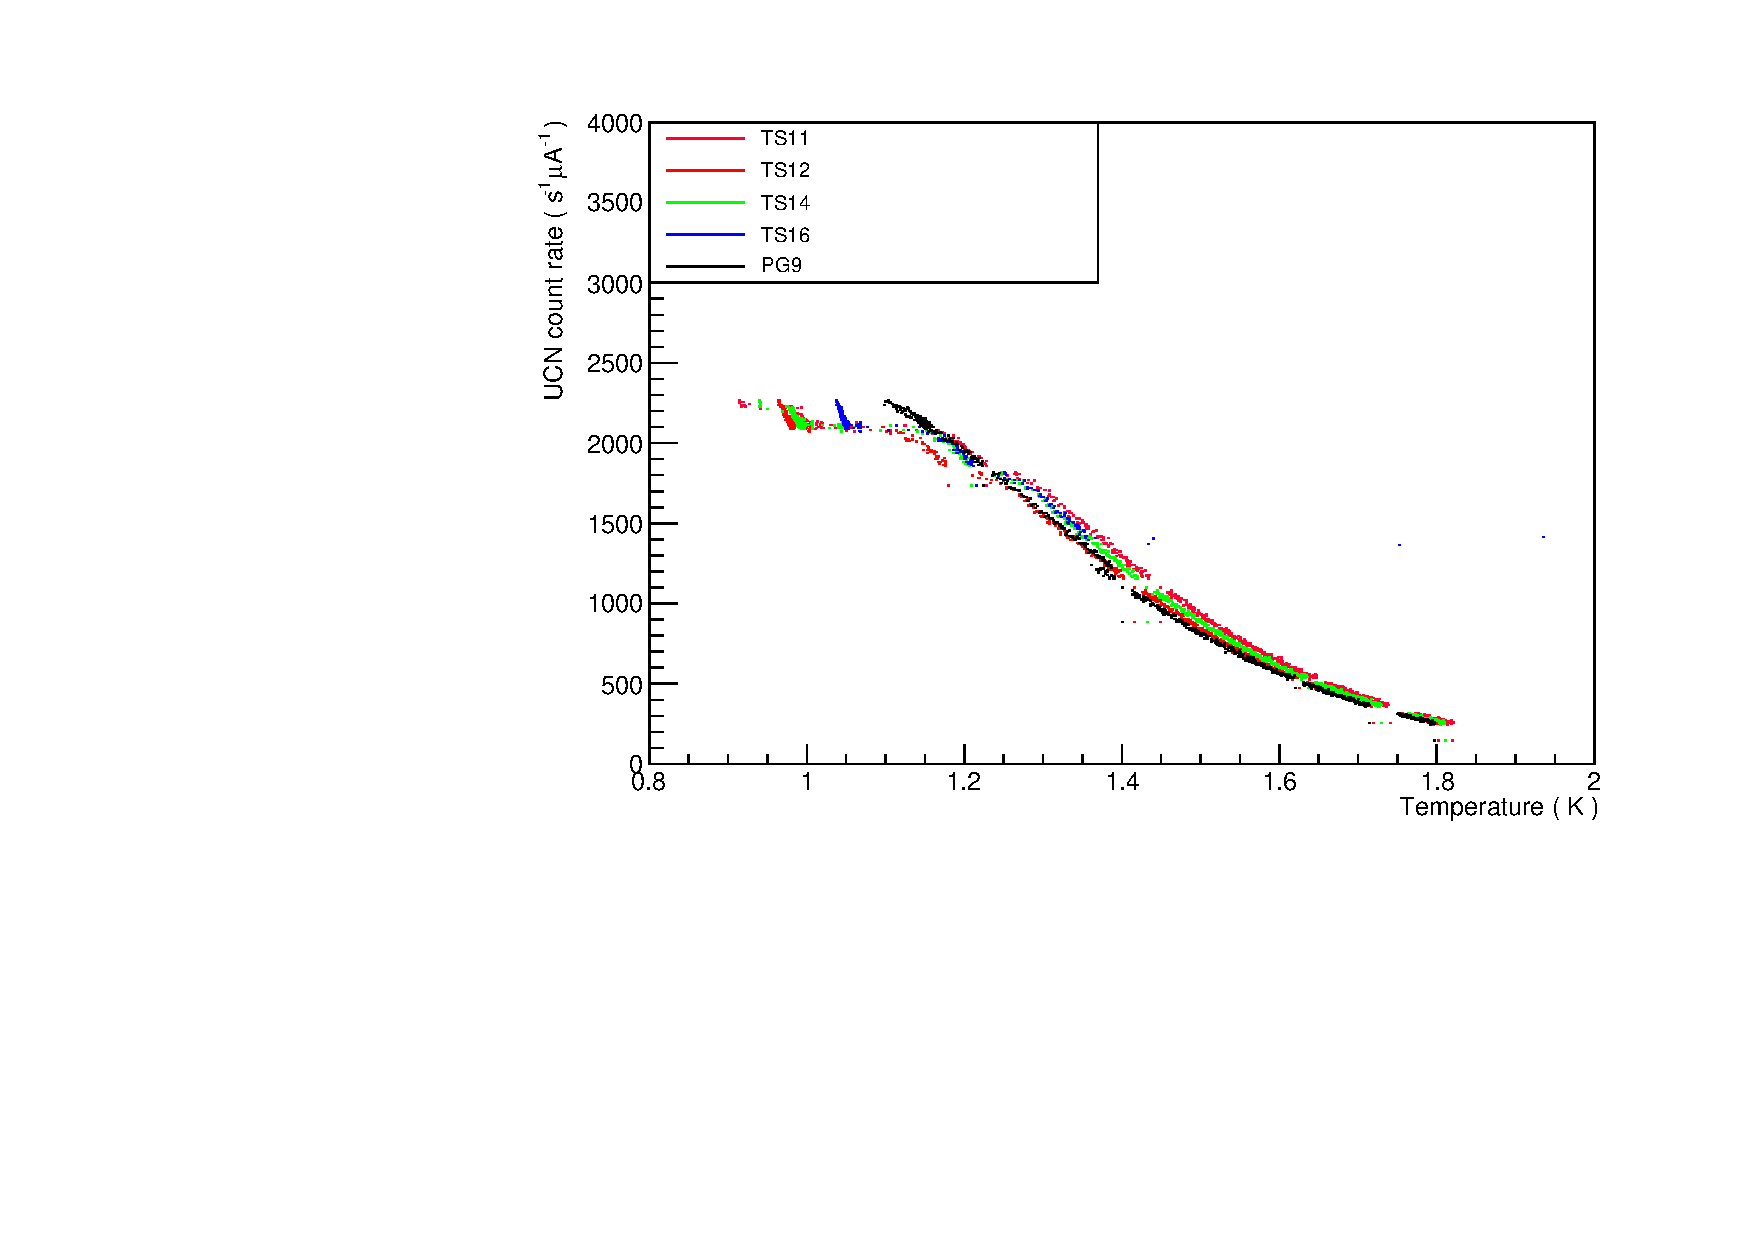
\includegraphics[width=\textwidth,page=1]{../steady_state/li6RateVsTempRun1162.pdf}
\caption{UCN count rates in the Li-6 detector during steady state warm-up}
\label{fig:steadyWarm}
\end{figure}

\begin{figure}
\centering
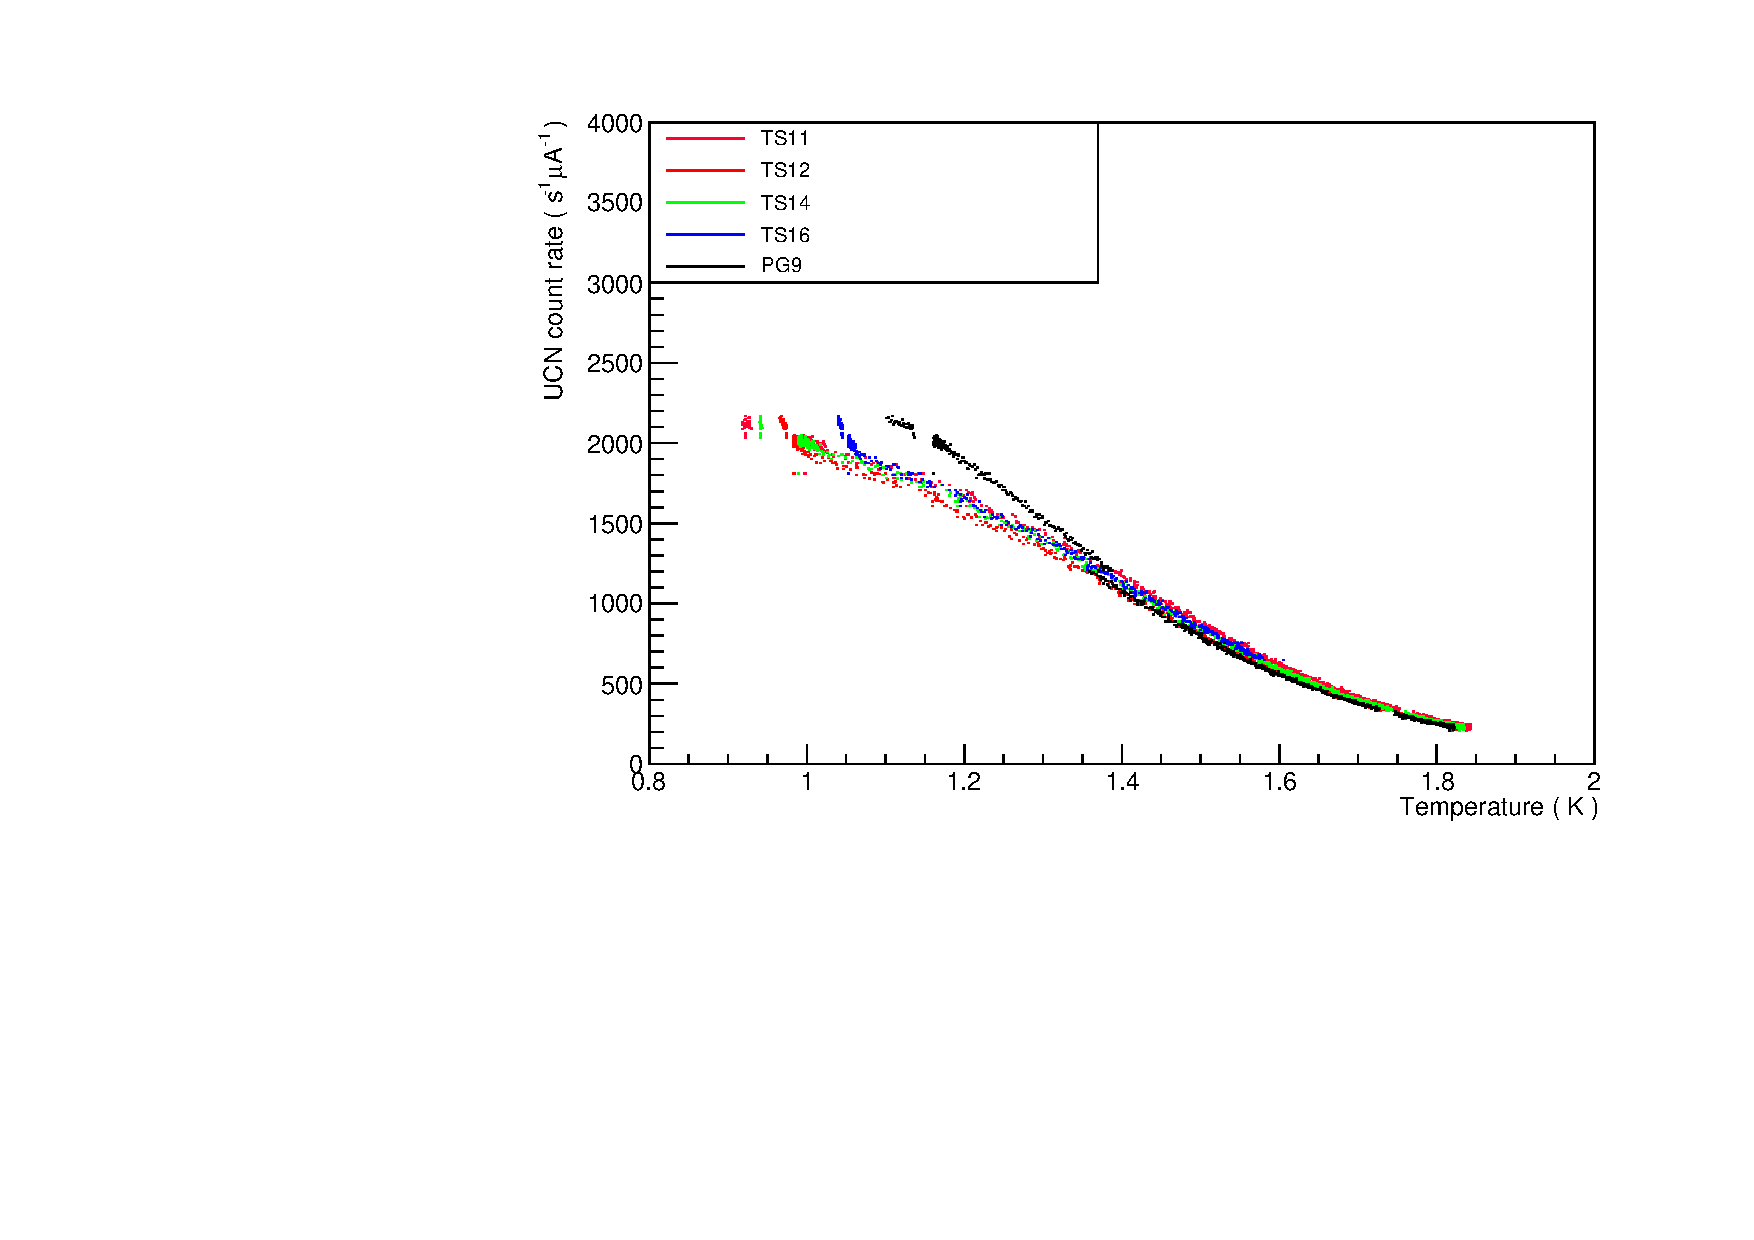
\includegraphics[width=\textwidth,page=1]{../steady_state/li6RateVsTempRun1163.pdf}
\caption{UCN count rates in the Li-6 detector during steady state cool-down}
\label{fig:steadyCool}
\end{figure}




\section{Storage lifetime in the source}




\section{Storage lifetime in guide components}




\section{Background rates}
\label{sec:background}



\section{Reproducibility}


\end{document}
